\graphicspath{{fig/model_fitting/}}

\chapter{Model fitting}	
\label{cha:model_fitting}

The task of a researcher working in the field of collective behaviour has to be in assessing the validity of proposed theoretical models. Models must be compared to real data. In this chapter we shall do exactly that: we shall generalise a popular model from the literature before proceeding to fit it to empirical data. Fitting is made in a Bayesian framework, which allows the capture of uncertainty in parameter estimation.

Though some work has been made at fitting theoretical models to field data, these attempts have typically used rudimentary methods to fit to some epiphenomena of the data, such as neighbour-density plots. Additionally, previous efforts have not made a systematic attempt at capturing uncertainty in parameter fitting --- capturing this uncertainty is especially important since typical datasets often have high levels of noise.

\section{Surf scoter dataset}
\label{sec:surf_data}

We were fortunate enough to receive a high quality dataset from a researcher in Canada \citep{lukeman10}. The dataset consists of $25$ sequences which describe the movements of surf scoters (a large sea duck) interacting on the surface of a lake. We are interested in this dataset because it provides tracking of individuals \emph{between} frames. Tracking individuals between frames is necessary to reproduce the trajectories of individuals.

\subsection{Visualisation}

The dataset was captured by fixing a camera at a vantage point above a lake and, in the presence of surf scoters, taking photographs every $3$ seconds. From the images, \citet{lukeman10} extracted the positions (recorded in pixel units) of agents in every frame. Every bird is assigned an ID number which allows the tracking of individuals between frames. The data extraction process is visualised in \cref{fig:lukeman_extraction}.

We received the dataset as $25$ arrays detailing the positions of every agent in every frame. Manually inspecting an array, however, does not give us much knowledge about the motion of the birds in that sequence. To counter this we produce animations of every sequence. (Digital) In \cref{anim:sequence05} we see an animation of the data contained in sequence $5$. The position of every agent in every frame is shown, along with its identification number.

Of course, animations aren't always an appropriate way to visualise sequences. Animations are particularly unhelpful when trying to showcase data in a static medium, such as a printed thesis, or a research paper. As such, we construct trajectory plots which attempt to show the same information as an animation does, but in a single image. Example trajectory plots are given in \cref{fig:seq05_traj}. For completeness, plots of all the sequences can be found in \cref{cha:data_plots}. These plots give us a general idea of the motion of the group in each sequence. We may also use these plots to highlight particular trajectories of interest, as in \cref{subfig:seq05_traj_highlight}. 

\begin{figure}[!tbp]
	\centering
	% http://mirror.ox.ac.uk/sites/ctan.org/macros/latex/contrib/movie15/doc/movie15.pdf for documentation
	\includemovie[attach=false,
				 depth=-175pt,
				 % Display an image to show before the video is played
				 text={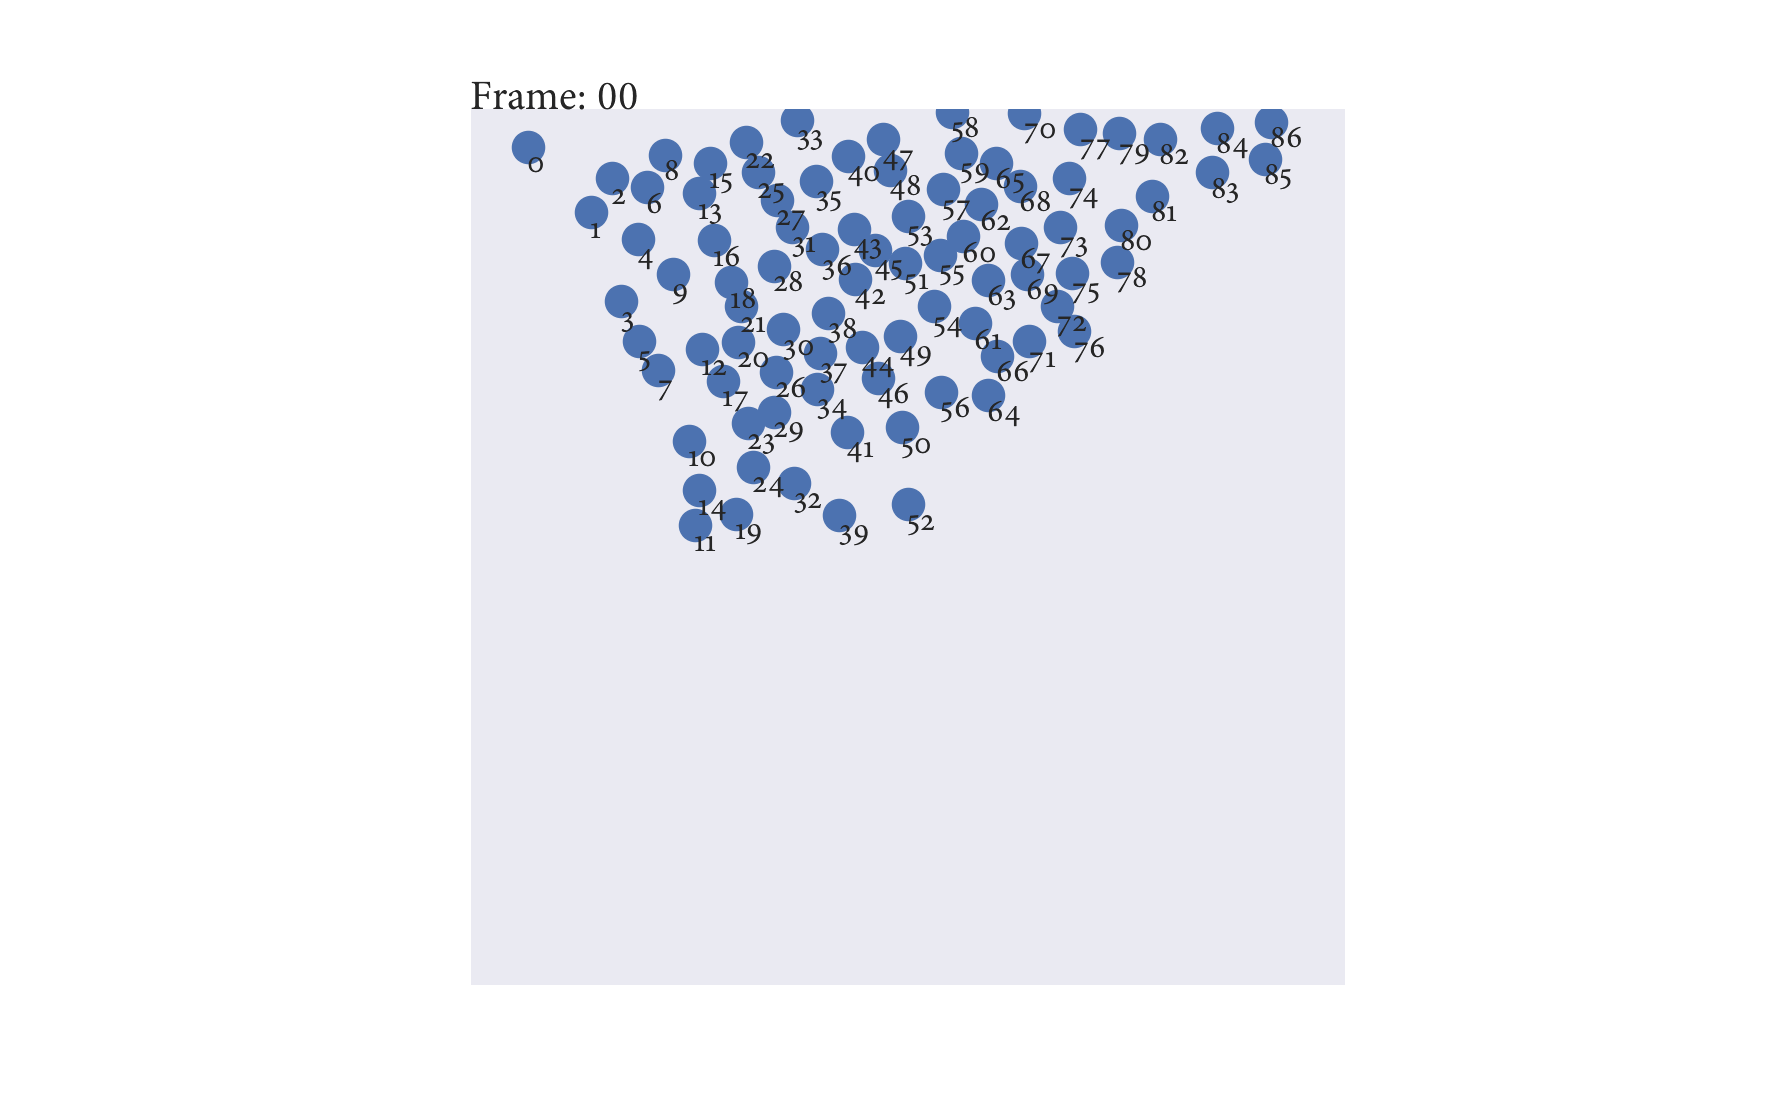
\includegraphics{/data/meetings/2018-06-11/sequence05frame00.png}},
				 repeat]
				 %{width}{height}{file}
				 {\textwidth}{\textwidth}{/data/surf_scoter/animate/sequence05.mp4}
	% Caption of video needs manual adjustment
	\vspace{-190pt}
	\caption{Animation of the data contained in sequence $5$. Each agent is annotated by its identifying number.}
	\label{anim:sequence05}
\end{figure}

\begin{figure}[!tbp]
	\begin{subfigure}[b]{0.5\textwidth}
		\centering
		\includegraphics{streamline_plots/sequence05.pdf}
		\caption{}
		\label{subfig:seq05_traj_no_highlight}
	\end{subfigure}%
	\begin{subfigure}[b]{0.5\textwidth}
		\centering
		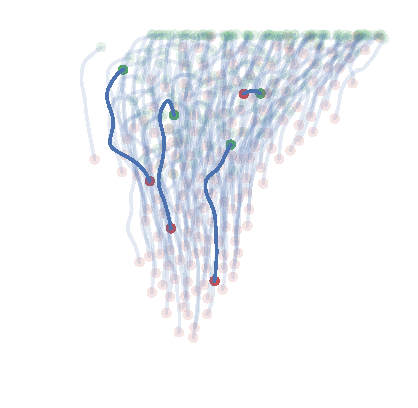
\includegraphics{streamline_plots/sequence05_highlight.pdf}
		\caption{}
		\label{subfig:seq05_traj_highlight}
	\end{subfigure}
	\caption{Inspecting the trajectories of the agents in sequence 5. The first observed positions of agents are represented by green markers. The last observed positions of agents are shown by red markers. \subref{subfig:seq05_traj_no_highlight}: The observed trajectories of all agents. \subref{subfig:seq05_traj_highlight}: Highlighting the observed trajectories of agents with ID $1$, $20$, $50$, $63$, $120$ and $155$.}
	\label{fig:seq05_traj}
\end{figure}

\subsection{Missingness}
\label{ssec:missingness}

At any given frame in a sequence there are individuals captured in the camera's field of vision, however, there are also individuals in the group which are not captured in the camera's view. We know that these uncaptured individuals exist as they may enter the field of vision at a later frame in the sequence, or we may have observed these individuals before they move out of the field of vision. As such, we know that there are individuals which may be influencing the group, which we don't observe in every frame. When an agent is missing from a frame, we say that this data is missing.

\begin{table}[!tbp]
		\pgfplotstabletypeset[col sep=&,
		% Set order of columns
		columns={number, numagents, numframes, begmiss, endmiss, totalmiss},
		columns/number/.style={
			column name={},
			column type=@{} >{\columncolor{white}[0pt][\tabcolsep]}c
			},
		columns/numagents/.style={
			column name={},
			column type=c
			},
		columns/numframes/.style={
			column name={}, 
			},
		columns/begmiss/.style={
			column name=Beginning,
			column type=@{}c,
			fixed, precision=0
			},
		columns/endmiss/.style={
			column name=End,
			column type=c,
			fixed, precision=0
			},
		columns/totalmiss/.style={
			column name=Total,
			column type=>{\columncolor{white}[\tabcolsep][0pt]}c@{},
			fixed, precision=0
			},
		every head row/.style={
			before row={
				\toprule
				% dec sep align splits columns in two to format, so there are really 6 data missing columns
				\multirow{2}{*}{Sequence} & \multirow{2}{*}{Agents} & \multirow{2}{*}{\hspace{0.2cm}Frames\hspace{0.4cm}} & \multicolumn{3}{c}{Data missing ($\%$)} \\
				\cmidrule{4-6}
				},
			after row={
				\midrule
				},
			},
%		every even row/.style={
%			before row={
%				\rowcolor{seaborn_face}
%				}
%			},
		every last row/.style={
			after row=\bottomrule
			}
	]
	{/data/thesis/tables/summary.csv}

		\caption{Summary of the  sequences in the dataset. Detailing the number of agents and the number
of frames in every sequence, as well as the amount of missing data.}
	\label{tab:summary_data}
\end{table}

We categorise an agent's missingness into two distinct categories: data missing in the \emph{beginning} of a sequence and data missing in the \emph{end} of a sequence. We say that an agent is missing in the beginning of a sequence if it is not observed in frame $0$, but is observed in some later frame number. Similarly, we say that an agent is missing in the end of a sequence if it is not observed in the final frame of the sequence, but was observed in some earlier frame. It is possible for an agent to have missingness both at the beginning \emph{and} the end of a sequence.

To get a general feel for the dataset and the information contained in each sequence, we summarise the data in \cref{tab:summary_data}. The sequences are labelled from sequence $1$ to sequence $25$, in order of increasing missingness. For each sequence we indicate the number of agents observed, the number of frames, and the percentage of data missing.

Though \cref{tab:summary_data} gives a general idea of how much data is missing in each sequence, it doesn't tell us how the missingness is distributed throughout the flock. For example, we still don't know whether the missingness is distributed uniformly throughout the flock or whether the majority of the missingess belongs to a minority of the flock. To help understand the distribution of missingness we created plots to visualise at which times every individual is and isn't observed. A sample of these constructed plots are shown in \cref{fig:missing}, and as before, plots of all the sequences are included in \cref{cha:data_plots}. A green grid point in the plot informs us that the bird with ID number $i$ was observed at frame $t$. Similarly, a red point shows us that bird $i$ was missing at frame $t$.

% **Manually** space figures to centre over subcaption because I have no self--respect
\begin{figure}[!tbp]
	\hfill
	\begin{subfigure}[b]{0.25\textwidth}
		\hspace{0.075cm}
		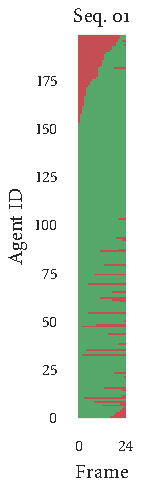
\includegraphics{missingness_plots/sequence01.pdf}
		\caption{}
		\label{subfig:missing1}
	\end{subfigure}%
	\hfill
	\begin{subfigure}[b]{0.25\textwidth}
		\hspace{0.3cm}
		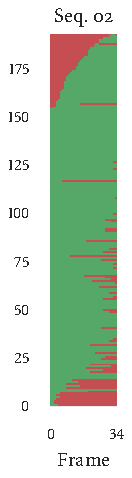
\includegraphics{missingness_plots/sequence02.pdf}
		\caption{}
		\label{subfig:missing2}
	\end{subfigure}%
	\hfill
	\begin{subfigure}[b]{0.25\textwidth}
		\hspace{0.35cm}
		\includegraphics{missingness_plots/sequence05.pdf}
		\caption{}
		\label{subfig:missing5}
	\end{subfigure}
	\hfill
	\caption{Visualisation of missingness in \subref{subfig:missing1} Sequence $1$ \subref{subfig:missing2} Sequence $2$ \subref{subfig:missing5} Sequence $5$. A green grid point tells us that agent $i$ was observed at frame $t$, and a red point tells us that agent $i$ was missing at time $t$.}
	\label{fig:missing}
\end{figure}

\section{Model development}
\label{sec:model_development}

Now that we have a feel for our dataset, we are ready to consider theoretical models which we can try fit to the data. There are many models which exist in the literature. In this section we shall describe one of the most popular models in the literature. Once described we shall consider how we can generalise this model to make it more flexible, and more biologically realistic. In this position, we are ready to fit this model to data.

\subsection{Vicsek Model}
\label{sec:vicsek_model}

\citet{vicsek95} devised a model which has now become a cornerstone of agent-based modelling. In their paper, \citet{vicsek95} showed that a simple model in which agents interact with neighbours only through alignment can produce movement reminiscent of real flocking behaviours. Furthermore, they showed the output of this model undergoes phase transitions as the amount of noise in the system is varied.

The Vicsek model simulates the movements of $N$ agents over $T$ timesteps. In the model agents seek to align their direction with that of their neighbours. Agents identify their neighbours as individuals which lie less than some fixed distance away. More formally, agent $i$'s neighbours at time $t$ are given by the set $n_{i,t} = \{\,j \mid d_{ij, t} < r, \, j=1,\ldots,N \,\}$, where $r$ is the interaction radius and $d_{ij, t}$ is the Euclidean-distance between agents $i$ and $j$ at time $t$.

Initially, agents are assigned a random position, $\bm{x}_{i, t=0}$, within a square cell of length $L$ and a random direction of motion $\theta_{i, t=0}$. Agents move with fixed speed $v$ and update their positions as
\begin{equation}\label{eq:pos_update}
	\bm{x}_{i, t+1} = \bm{x}_{i, t} + \bm{v}_{i, t},
\end{equation}
where $\bm{v}_{i, t}$ is constructed to have direction $\theta_{i, t+1}$ and magnitude $|\bm{v}_{i, t}| = v$.

An agents directional update is computed as the average direction of its neighbours plus some noise term. To compute the average direction, we refer to circular mean defined in \cref{eq:circ_mean}. With this definition, we can compute the average direction of agent $i$'s neighbours at time $t$ as
\begin{equation}
\label{eq:vicsek_average}
	\langle \theta \rangle_{i, t} = \atantwo \bigg( \frac{1}{|n_{i, t}|} \sum_{j=1}^N \mathds{1}_{n_{i, t}}(j) \sin{\theta_{j ,t}}, \frac{1}{|n_{i, t}|} \sum_{j=1}^N \mathds{1}_{n_{i, t}}(j)  \cos{\theta_{j, t}} \bigg),
\end{equation}
where the indicator function, $\mathds{1}$ , is defined
\begin{equation*}
	\mathds{1}_{n_{i, t}}(j) =
	\begin{cases}
		1 & \text{ if } j \in n_{i, t} \\
		0 & \text{ if } j \notin n_{i, t}.
	\end{cases}
\end{equation*}

The noise in Vicsek's model was drawn from a uniform $U(-\eta/2, \eta/2)$ distribution and summed with the average direction. Putting this all together allows us to realise agent $i$'s directional update as
\begin{equation}
\label{eq:vicsek_update}
	\theta_{i,t+1} \mid \langle \theta \rangle_{i, t}, \eta \sim U\big(\langle \theta \rangle_{i, t} -\eta/2, \langle \theta \rangle_{i, t} + \eta/2\big).
\end{equation}

\subsection{Hierarchical Vicsek}
\label{ssec:general_vicsek}

Here we shall seek to alter the Vicsek model so that it becomes more biologically realistic. One of the ways we do this is by introducing hierarchy into the model, which allows variation within groups. 

In all of the agent-based models encountered in the literature, there is no inter-agent variation --- all the agents in a group are identical. In the context of the Vicsek model, all the agents have the same interaction radius $r$, and are all subjected to noise generated from a uniform $U(-\eta/2, \eta/2)$ distribution. In affect, the individuals in the groups respond identically to the same stimulus.

% Couzin's leader follower work is the only model I can think of where all the agents don't behave identically

In reality, there will be biological and behavioural variation within groups of individuals. Some individuals may be more prone to noise, others less. Similarly, some agents may pay close attention to the movements of their neighbours, whereas other individuals may pay less attention. These differing responses may be due to physiological differences between the individuals, but they also may be linked to social hierarchy, or correlated with the age and experience of an individual. With these considerations, we conclude that we should allow variation within groups. In Vicsek, we do so by assigning every agent its own interaction radius $r_i$, and allowing individuals to be more or less prone to noise, assigning each agent its own parameter $\eta_i$.

In considering the Vicsek model, we decide that the hard cut-off imposed by the interaction radius $r_i$ is biologically unrealistic. In this paradigm, interactions are binary: agents interact fully, or not at all. For example, consider that the distance between agent $i$ and $j$ at time $t$ is  $r_i + |\, \epsilon \,|$, for $|\, \epsilon \, | \ll 1$. In this case agent $j$ makes no contribution to agent $i$'s direction. However, if $d_{ij, t} = r_i - |\, \epsilon\,| $ for $|\, \epsilon \,| \ll 1$, then agent $j$ makes a full contribution to agent $i$'s direction. This case is visualised in \cref{subfig:no_interact}. Similarly, because of the interaction, agents distanced $|\,\epsilon\,|$ and $r_i - |\,\epsilon\,|$ away from agent $i$, both influence agent $i$ equally.

\begin{figure}[!tbp]
	\begin{subfigure}[b]{0.45\textwidth}
		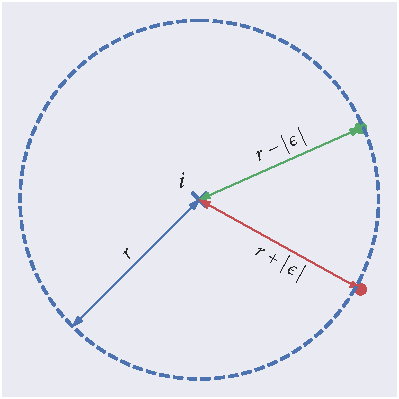
\includegraphics{no_interact.pdf}
		\caption{}
		\label{subfig:no_interact}
	\end{subfigure}%
	\hspace{0.05\textwidth}
	\begin{subfigure}[b]{0.45\textwidth}
		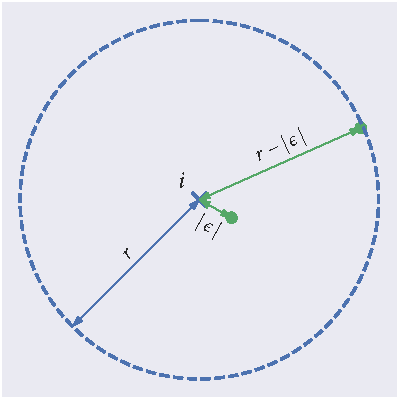
\includegraphics{interact.pdf}
		\caption{}
		\label{subfig:interact}
	\end{subfigure}
	\caption{Agent $i$, its interaction radius and neighbours (green). \subref{subfig:no_interact}: The hard cut-off at $r$. \subref{subfig:interact}: Without weighting both neighbours influence $i$ equally.}
\end{figure}

Our belief is that the averaging process should be weighted by distance. That way, a neighbour very close to agent $i$ will have more influence than a neighbour much further away. We decide that a bivariate normal distribution provides an appropriate weighting function. We calculate $\omega_{ij, t}$, the weighting which agent $i$ will give to neighbour $j$'s direction at time $t$, defined by the bivariate normal distribution with mean $(x_{i, t}, y_{i, t})^T$ and covariance
\[
	\Sigma_i = \begin{bmatrix}
		\sigma_{X_i}^2 & 0 \\
		0 & \sigma_{X_i}^2
	\end{bmatrix}.
\]
Now, we can adapt \cref{eq:vicsek_average} to define the weighted average:
\begin{equation}
\label{eq:weighted_average}
	\langle \theta \rangle_{i, t} = \atantwo \bigg( \frac{1}{N} \sum_{j=1}^N \omega_{ij, t} \sin{\theta_{j ,t}}, \frac{1}{N} \sum_{j=1}^N \omega_{ij, t} \cos{\theta_{j, t}} \bigg).
\end{equation}

The final refinement which we make is to alter the distribution from which the noise is generated. In Vicsek noise is generated from a uniform distribution, so agents are just as likely to be perturbed by large amounts of noise as small amounts. We consider that the likelihood of experiencing a particular noise term should be weighted by the magnitude of the noise, and that small noise terms should be encountered more frequently than large noise terms. To account for this we generate noise from a normal $\Normal(0, \sigma_{Y_i})$. In our modified model, agents update their direction according to
\begin{equation}
\label{eq:weighted_update}
	\theta_{i,t+1} \mid \langle \theta \rangle_{i, t}, \sigma_{Y_i} \sim \Normal\big(\langle \theta \rangle_{i, t}, \sigma_{Y_i}\big).
\end{equation}

In our adapted version of Vicsek's model, agent $i$'s behaviour is controlled by the parameters $\sigma_{X_i}$ and $\sigma_{Y_i}$. The weighting which agent $i$ gives to its neighbours depends on the $\sigma_{X_i}$; a large value of $\sigma_{X_i}$ corresponds to an agent which weights its neighbours strongly, and a small value of $\sigma_{X_i}$ corresponds to an agent which pays little attention to its neighbours. Similarly, the parameter $\sigma_{Y_i}$ controls how much noise an agent experiences. A large value of $\sigma_{Y_i}$ corresponds to an agent which experiences large amounts of noise. In a similar manner, a small value of $\sigma_{Y_i}$ tells us that agent $i$ is only perturbed by small amounts.

With the parameters of the model decided, we are left to choose appropriate hyperparameters. In both cases our parameters are standard deviations, and so are strictly positive. This should be reflected in the distributions over these parameters. We decide to use gamma distributions in both cases as it has support $(0, \infty)$.

Typically, the gamma distribution is parameterised as $\Ga(g, h)$. Here, however, we opt to parameterise the gamma distribution by its mean and variance. Given that $\bm{X} \given g, h \sim \Ga(g, h)$, it is known that $\textrm{E}[\bm{X}] = g / h$ and $\textrm{Var}(\bm{X}) = g/h^2$. Letting $m = \textrm{E}[\bm{X}]$ and $v =\textrm{Var}(\bm{X})$, we see that $g = m^2 / v$ and $h = m / v$. As such, we see that an alternative, yet equivalent parameterisation is $\bm{X} \given m, v \sim \Ga(m^2 / v, m / v)$. We prefer this parameterisation as constructing prior distributions over $m$ and $v$ is more intuitive than working with $g$ and $h$. Putting all this together, we decide that the interaction parameter should be distributed as
\begin{equation}
	\label{eq:x_hypers}
	\bm{\sigma}_X \given m_X, v_X \sim \Ga(m_X^2 / v_X, m_X / v_X).
\end{equation}
Similarly, for the noise parameter we stipulate the distribution
\begin{equation}
	\label{eq:y_hypers}
	\bm{\sigma}_Y \given m_Y, v_Y \sim \Ga(m_Y^2 / v_Y, m_Y / v_Y).
\end{equation}

\section{Inferring parameters}
\label{sec:vicsek_infer}

With the model setup, we are now ready to fit this model to the dataset described in \cref{sec:surf_data} and perform parameter inference. To use the inference methods introduced in \cref{cha:bayes_intro}, we need to able to express the likelihood of the parameters given some data. 

Let us begin by considering the likelihood of observing a single agent update its direction, in the presence of neighbours, from $\theta_{i, t}$ to $\theta_{i, t+1}$. Using \cref{eq:weighted_update}, $\sigma_{X_i}$ and $\{\theta_{j, t}, \bm{x}_{j, t} \mid j=1,\ldots,N\}$ to compute the mean direction $\langle \theta \rangle_{i, t}$, we may realise the likelihood:
\begin{equation}
\label{eq:simple_likelihood}
	L\big(\sigma_{X_i}, \sigma_{Y_i} \given \theta_{i, t+1},  \{\,\theta_{j, t}, \bm{x}_{j, t} \mid j=1,\ldots,N\,\}\big) = \bigg( \frac{1}{2\pi\sigma_{Y_i}^2} \bigg)^{1/2} \exp{-\frac{1}{2\sigma_{Y_i}^2} \bigg(\theta_{i, t+1} - \langle \theta \rangle_{i, t}\bigg)^2 }.
\end{equation}

% Is the prime on the t necessary? Just didn't really like t=t,t+1.
Let us now consider that we wish to compute the likelihood of observing agent $i$'s directions $\theta_{i, t}$, $\theta_{i, t+1}$ and $\theta_{i, t+2}$, again in the presence of neighbours. Using that successive noise terms are independent, we can express the likelihood as a product
\begin{align*}
	& L\big(\sigma_{X_i}, \sigma_{Y_i}  \given \theta_{i, t+2},  \{\,\theta_{j, t'}, \bm{x}_{j, t'} \mid j=1,\ldots,N, \, t'=t,t+1\,\}\big) \\
									& = L(\sigma_{X_i}, \sigma_{Y_i} \given \theta_{i, t+2}, \{\, \theta_{j, t+1}, \bm{x}_{j, t+1} \mid j=1,\ldots,N\,\} \bigcdot L(\sigma_{X_i}, \sigma_{Y_i} \given \theta_{i, t+1}, \{\, \theta_{j, t}, \bm{x}_{j, t} \mid j=1,\ldots,N\,\}.
\end{align*}
We may notice that the two terms in the product are of the same form as in \cref{eq:simple_likelihood}. Using this observation, we rewrite the likelihood more compactly
\begin{align*}
L\big(\sigma_{X_i}, \sigma_{Y_i}  \given \theta_{i, t+2},  \{\,\theta_{j, t'}, \bm{x}_{j, t'} \mid j=1,\ldots,&N, \, t'=t,t+1\,\}\big) \\
& = \prod_{t'=t}^{t+1} L\big(\sigma_{X_i}, \sigma_{Y_i} \given \theta_{i, t+1},  \{\,\theta_{j, t}, \bm{x}_{j, t} \mid j=1,\ldots,N\,\}\big) \\
& = \prod_{t'=t}^{t+1} \bigg( \frac{1}{2\pi\sigma_{Y_i}^2} \bigg)^{1/2} \exp{-\frac{1}{2\sigma_{Y_i}^2} \bigg(\theta_{i, t+1} - \langle \theta \rangle_{i, t}\bigg)^2 }
\end{align*}

Using the product notation makes it much easier to express and evaluate likelihoods of data over many timesteps. For example, suppose that we now observe the movements of $N$ agents from timestep $t=1$ to timestep $t=T$. The likelihood of observing agent $i$'s trajectory can be neatly expressed
\begin{align*}
	L\big(\sigma_{X_i}, \sigma_{Y_i}  \given \theta_{i, T},  \{\,\theta_{j, t}, \bm{x}_{j, t} \mid j= 1,\ldots,&N, \, t=1,  \ldots,T-1\,\}\big) \\
	& = \prod_{t=1}^{T-1} L\big(\sigma_{X_i}, \sigma_{Y_i} \given \theta_{i, t+1},  \{\,\theta_{j, t}, \bm{x}_{j, t} \mid j=1,\ldots,N\,\}\big) \\
	& = \prod_{t=1}^{T-1} \bigg( \frac{1}{2\pi\sigma_{Y_i}^2} \bigg)^{1/2} \exp{-\frac{1}{2\sigma_{Y_i}^2} \bigg(\theta_{i, t+1} - \langle \theta \rangle_{i, t}\bigg)^2 }.
\end{align*}

Realising the likelihood of observing the movements of multiple agents is a similar process to expressing the likelihood of a single agent over multiple steps. First, we must recognise that the noise terms experienced by agents $i$ and $i+1$ are independent and that this allows the likelihood to be factorised as a product over the agents. With this acknowledgement, we determine that the likelihood of observing the movements of $N$ agents over $T$ timesteps, given the parameters $\bm{\sigma}_X$ and $\bm{\sigma}_Y$, to be
\begin{align}
\label{eq:data_likelihood}
\begin{split}
	L\big(\bm{\sigma}_X, \bm{\sigma}_Y  \given \{\,\theta_{i, T} \mid i=1,\ldots,N\,\},  \{&\,\theta_{j, t}, \bm{x}_{j, t} \mid j= 1,\ldots, N, \, t=1,  \ldots,T-1\,\}\big) \\
	& = \prod_{i=1}^N \prod_{t=1}^{T-1} L\big(\sigma_{X_i}, \sigma_{Y_i} \given \theta_{i, t+1},  \{\,\theta_{j, t}, \bm{x}_{j, t} \mid j=1,\ldots,N\,\}\big) \\
	& = \prod_{i=1}^N \prod_{t=1}^{T-1} \bigg( \frac{1}{2\pi\sigma_{Y_i}^2} \bigg)^{1/2} \exp{-\frac{1}{2\sigma_{Y_i}^2} \bigg(\theta_{i, t+1} - \langle \theta \rangle_{i, t}\bigg)^2 }.
\end{split}
\end{align}

So, we can now express the likelihood of the data, given the parameters $\bm{\sigma}_X$ and $\bm{\sigma}_Y$. Recall, however, that there is still the matter of the hyperparameters to be considered. Revisiting \cref{eq:x_hypers,eq:y_hypers} allows us to formulate the likelihood of the hyperparameters, given the parameters, as a product of successive evaluations of the Gamma distribution:
\begin{equation}
\label{eq:param_likelihood}
	L(m_X, v_X, m_Y, v_Y \given \bm{\sigma}_X, \bm{\sigma}_Y) = \prod_{i=1}^N \frac{h_X^{g_X}}{\Gamma(g_X)} \sigma_{X_i}^{g_X - 1} \exp{-h_X \sigma_{X_i}}  \prod_{i=1}^N \frac{h_Y^{g_Y}}{\Gamma(g_Y)} \sigma_{Y_i}^{g_Y - 1} \exp{-h_Y \sigma_{Y_i}},
\end{equation}
where $g_X = m_X^2 / v_X$, $h_X = m_X / v_X$, and similarly for $g_Y$ and $h_Y$.

We are now in a position to express the likelihood of observing data describing the movements of $N$ agents over $T$ timesteps, given parameters $\bm{\sigma}_X$, $\bm{\sigma}_Y$ and hyperparameters $m_X$, $v_X$, $m_Y$ and $v_Y$, combining \cref{eq:data_likelihood,eq:param_likelihood} to see
\begin{align}
\label{eq:full_likelihood}
\begin{split}
& 	L\big(m_X, v_X, m_Y, v_Y, \bm{\sigma}_X, \bm{\sigma}_Y  \given \{\,\theta_{i, T} \mid i=1,\ldots,N\,\},  \{\,\theta_{j, t}, \bm{x}_{j, t} \mid j= 1,\ldots, N, \, t=1,  \ldots,T-1\,\}\big) \\
	& = 	L(m_X, v_X, m_Y, v_Y \given \bm{\sigma}_X, \bm{\sigma}_Y)\\
	& \qquad\qquad\qquad \!\! \bigcdot L\big(\bm{\sigma}_X, \bm{\sigma}_Y  \given \{\,\theta_{i, T} \mid i=1,\ldots,N\,\},  \{\,\theta_{j, t}, \bm{x}_{j, t} \mid j= 1,\ldots, N, \, t=1,  \ldots,T-1\,\}\big)\\
	& = \prod_{i=1}^N \frac{h_X^{g_X}}{\Gamma(g_X)} \sigma_{X_i}^{g_X - 1} \exp{-h_X \sigma_{X_i}} \prod_{i=1}^N  \frac{h_Y^{g_Y}}{\Gamma(g_Y)} \sigma_{Y_i}^{g_Y - 1} \exp{-h_Y \sigma_{Y_i}}\\
	& \qquad\qquad\qquad \!\! \bigcdot \prod_{i=1}^N \prod_{t=1}^{T-1} \bigg( \frac{1}{2\pi\sigma_{Y_i}^2} \bigg)^{1/2} \exp{-\frac{1}{2\sigma_{Y_i}^2} \bigg(\theta_{i, t+1} - \langle \theta \rangle_{i, t}\bigg)^2 }.
\end{split}
\end{align}

Now, to write down the full posterior distribution we need only combine the likelihood of \cref{eq:full_likelihood} with prior beliefs $\pi(m_X, v_X, m_Y, v_Y)$. Again, because we are considering the mean and variance of standard deviations, we chose to represent our prior beliefs with Gamma distributions. We consider that that our prior beliefs between mean and variance are independent, and so express the hyperprior as
\begin{equation*}
	\pi(m_X, v_X, m_Y, v_Y) = \pi(m_X) \pi(v_X) \pi(m_Y) \pi(v_Y).
\end{equation*}
We then write down our prior beliefs on each of the hyperparameters separately
\begin{align*}
	m_X \given \alpha_X, \beta_X & \sim \Ga(\alpha_X, \beta_X) \\
	v_X \given \lambda_X, \gamma_X & \sim  \Ga(\lambda_X, \gamma_X) \\
	m_Y \given \alpha_Y, \beta_Y & \sim \Ga(\alpha_Y, \beta_Y) \\
	v_Y \given \lambda_Y, \gamma_Y & \sim  \Ga(\lambda_Y, \gamma_Y),
\end{align*}
where the parameters $\bm{\alpha}$, $\bm{\beta}$, $\bm{\lambda}$ and $\bm{\gamma}$ are to be chosen later.

\section{Inferring missingness}
\label{ssec:vicsek_paths}

% Detail proposal scheme etc.

In \cref{ssec:missingness} we considered that there are missing data points in the sequences. In total, $28\%$ of the dataset is missing from sequence $5$. Of this missing data, $3\%$ is missing at the end of the sequence and $25\%$ is missing in the beginning of the sequence. In total there are a possible $5\,301$ datapoints in the sequence, of which $1\,468$ points are missing.

We handle the missingness by integrating over all the possible paths an agent could have made when unobserved. The handling of the missing data is more computationally intensive than inferring the parameters of the model as the dimensionality of the missing data is ($\approx 5 \times$) bigger. As such, this part of the inference scheme is inferring a very large amount of data. \emph{In the future I will detail the proposal mechanisms I used to propose missing directions at the beginning and end of the sequences (the cases are handled separately), and the resulting corrections to the acceptance ratio.}

\section{Output}
\label{ssec:vicsek_params}

Inference shall be made only on sequence $5$ (\emph{in time we will extend our inference to work on all the sequences}). We chose this sequence as there is more perturbation in the trajectories of this sequence than some of the other sequences. We understand that the more the trajectories of the agents depart from a straight line, the more information that sequence contains.

The behaviour of every agent in the model is specified by two parameters. In total, sequence $5$ tracks the movements of $171$ agents --- this means there are $342$ parameters to fit in this sequence. In addition to the parameters, there are a further $4$ hyperparameters. Our scheme will therefore need to explore a parameter space with $346$ dimensions. For now, we shall concentrate only on the parameters in the model, and not consider the missingness.

We run Metropolis-Hastings as described in \cref{alg:metropolis_hastings}, for $10^6$ iterations, thinning the output by a factor of $100$. We perform a normal random walk to explore the parameter space. To help the mixing of the chains over such a large parameter space, the space is divided into three blocks, containing the hyperparmaeters, $\sigma_X$ and $\sigma_Y$ parameters separately.

A run of this scheme took approximately $11$ hours to complete. Evaluating the likelihood is computationally expensive as to explore the parameter space of $\bm{\sigma}_X$ we are required to recompute $\langle \theta \rangle_{i, t}$ for $i=1,\ldots,175$, $t=1,\ldots,31$ at every iteration --- of which there were $10^6$. Of the proposed parameters $27\%$ of the hyperparameters, $19\%$ of the $\bm{\sigma}_X$ parameters, and $29\%$ of $\bm{\sigma}_Y$ parameters were accepted.

A selection of the output from the scheme is visualised in \crefrange{fig:trace_hyper}{fig:hist_sigmax}. In these plots we see that the chains over the hyperparameters have converged. Of particular note is $v_X$ --- we see from \cref{fig:hist_hyper} that this inferred value is very large, suggesting that there is a lot of variation in the $\sigma_X$ parameters and how the individuals in the group interact with their neighbours. It appears that some agents are interacting more strongly with neighbours than others. This appears an interesting result, contradicting the assumption of many models in the literature that all agents behave identically.

From \cref{fig:trace_sigmay,fig:hist_sigmay} we see that our chains over the $\sigma_Y$ parameters have almost converged --- though our scheme would benefit from a slightly longer run with more thinning. Recall that $\sigma_{Y_i}$ determines how much noise is experienced by agent $i$. To help interpret this parameter, we take the mean value over each of the first four $\sigma_Y$ chains. In \cref{fig:noise_pdf} we plot normal distributions with standard deviations set by the mean of these chains. We immediately get a sense that the noise terms which agents experience are very small. To further help us interpret the noise terms we plot polar histograms of draws from these distributions in \cref{fig:noise_polar}.

Looking at the chains over the first four $\sigma_X$ parameters and the corresponding posterior beliefs, given in \cref{fig:trace_sigmax,fig:hist_sigmax} respectively, we see that our chains have not finished converging. To reach convergence our scheme needs running for longer with more thinning applied. (Alternatively we could attempt to tune the random walk better, after all the acceptance rate of the $\sigma_X$ chains was $0.19$, which is a little low.)  Despite this, we can see that our chains are beginning to converge. \emph{It is not obvious how to interpret the $\sigma_X$ parameters --- we have tried a few approaches. I shall omit them for now until we are completely satisfied with the measures we use.}

\begin{figure}[tbp]
	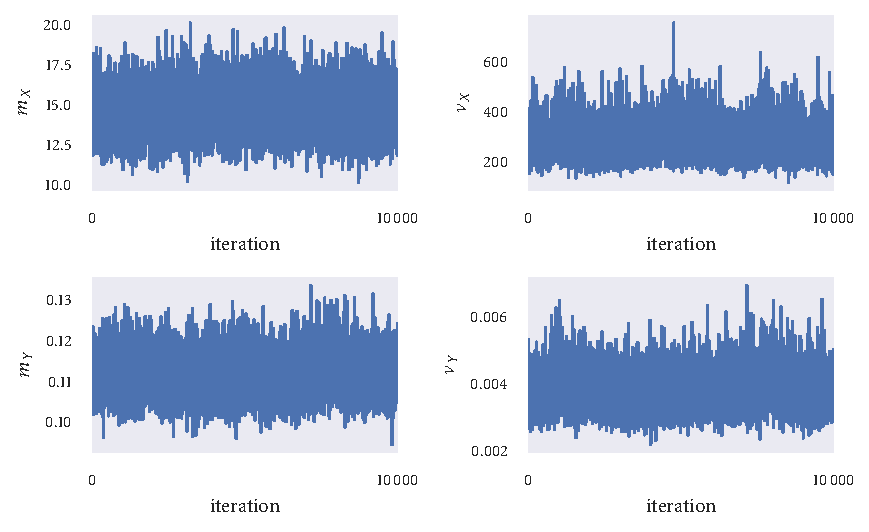
\includegraphics{seq05_trace_hyper.pdf}
	\caption{Trace plots over the hyperparameters.}
	\label{fig:trace_hyper}
\end{figure}
\begin{figure}[bp]
	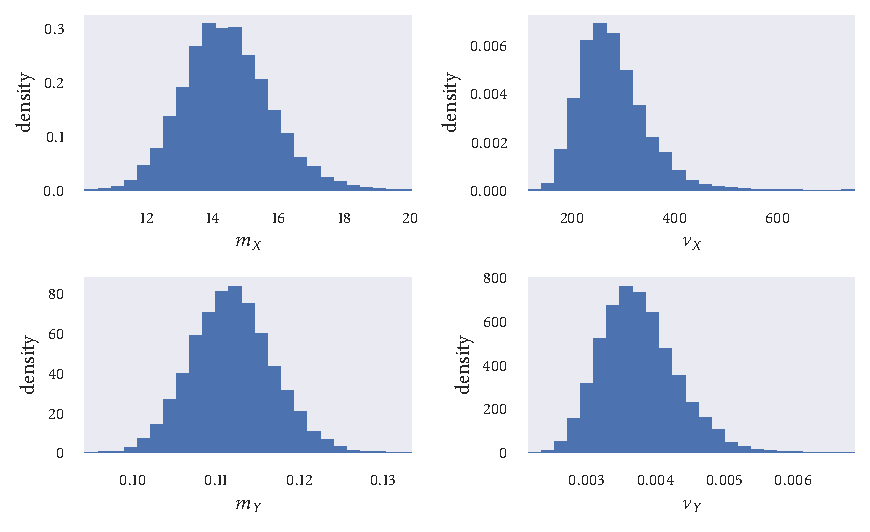
\includegraphics{seq05_hist_hyper.pdf}
	\caption{Histogram plots of our posterior beliefs about the hyperparameters $m_X$, $v_X$, $m_Y$ and $v_Y$.}
	\label{fig:hist_hyper}
\end{figure}
\begin{figure}[!tbp]
	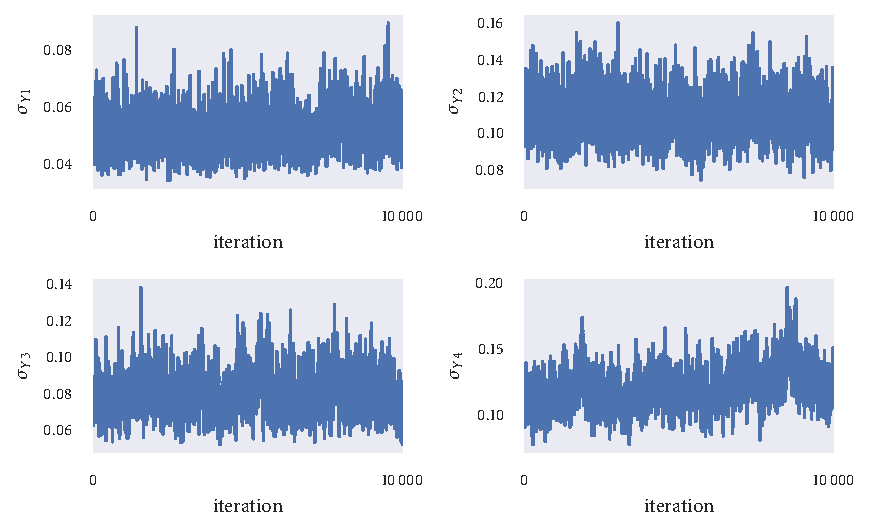
\includegraphics{seq05_trace_sigmay.pdf}
	\caption{Trajectories of the chains over the first four $\sigma_Y$ parameters.}
	\label{fig:trace_sigmay}
\end{figure}
\begin{figure}[!tbp]
	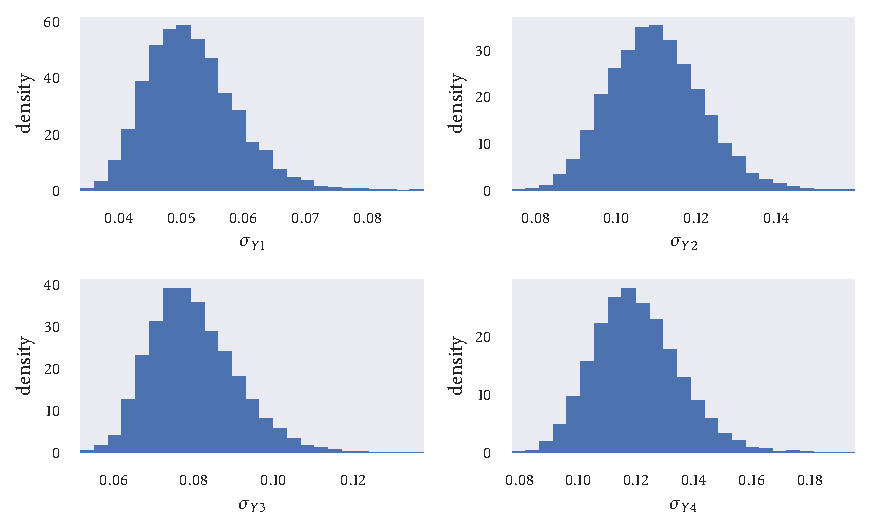
\includegraphics{seq05_hist_sigmay.pdf}
	\caption{Posterior beliefs about the parameters $\sigma_{Y_1}$, $\sigma_{Y_2}$, $\sigma_{Y_3}$ and $\sigma_{Y_4}$.}
	\label{fig:hist_sigmay}
\end{figure}
\begin{figure}[!tbp]
	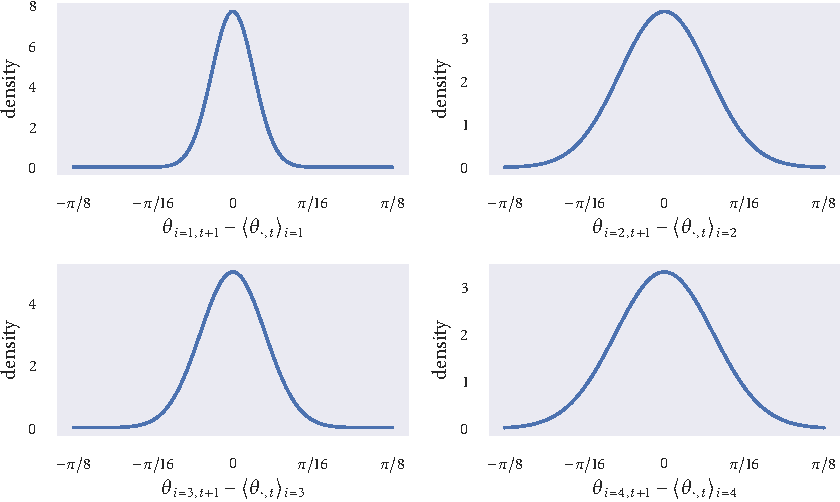
\includegraphics{/data/meetings/2018-04-30/noise_plot.pdf}
	\caption{Taking the mean values of the chains over $\sigma_{Y_1}$, $\sigma_{Y_2}$, $\sigma_{Y_3}$ and $\sigma_{Y_4}$, here we plot the noise experienced by agents $1$, $2$, $3$ and $4$.}
	\label{fig:noise_pdf}
\end{figure}
\begin{figure}[!tbp]
	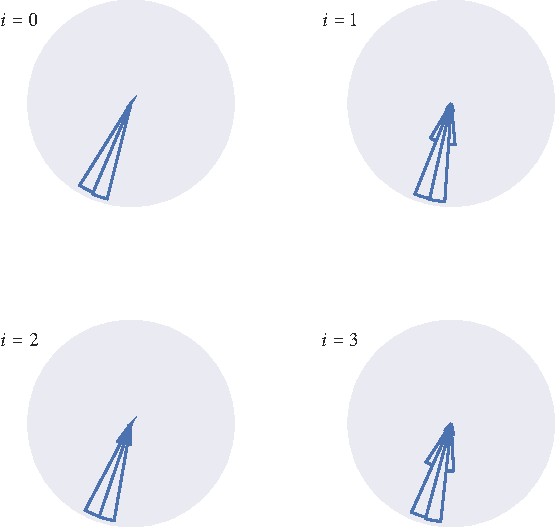
\includegraphics{/data/meetings/2018-05-28/seq05_polar_noise.pdf}
	\caption{The noise experienced by agents $1$, $2$, $3$ and $4$, plotted on polar histograms, rotated by the average direction of each agent throughout the sequence.}
	\label{fig:noise_polar}
\end{figure}
\begin{figure}[!tbp]
	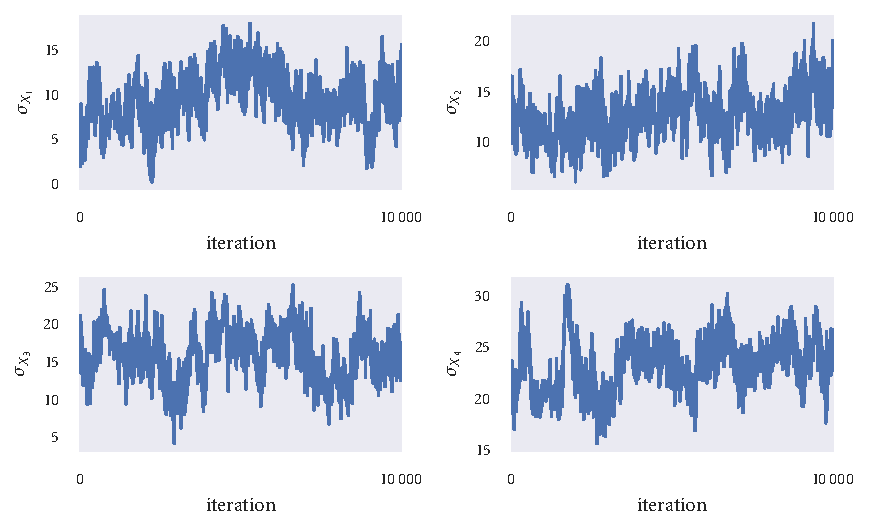
\includegraphics{seq05_trace_sigmax.pdf}
	\caption{Chains over the parameters $\sigma_{X_1}$, $\sigma_{X_2}$, $\sigma_{X_3}$ and $\sigma_{X_4}$.}
	\label{fig:trace_sigmax}
\end{figure}
\begin{figure}[!tbp]
	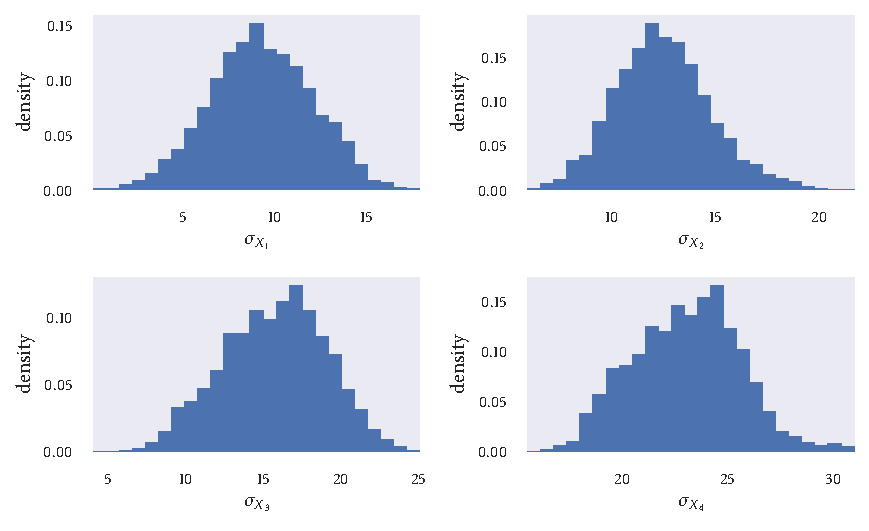
\includegraphics{seq05_hist_sigmax.pdf}
	\caption{Samples from the posterior distribution over the first four $\sigma_X$ parameters.}
	\label{fig:hist_sigmax}
\end{figure}

Of the paths proposed at the end of the sequence $100\%$ are accepted. However, for the paths proposed at the beginning of the scheme only $17\%$ are accepted. The scheme took a little over $8$ hours to run.

Because we are inferring such a large amount of data it is infeasible to assess all of the output visually. Here we shall inspect a small amount of the inferred data. \cref{fig:seq05_trace_end_miss_i=17,fig:seq05_hist_end_miss_i=17,fig:seq05_polar_hist_end_miss_i=17} visualise inferred data at the end of the sequence. In particular, these plots assess the inferred directions of bird $17$ over frames $1$, $2$, $3$ and $4$. The chains shown in \cref{fig:seq05_trace_end_miss_i=17} show that our scheme has here converged, and in \cref{fig:seq05_hist_end_miss_i=17,fig:seq05_polar_hist_end_miss_i=17} we inspect our posterior beliefs about the missing directions.

In \cref{fig:seq05_trace_beg_miss_i=97,fig:seq05_hist_beg_miss_i=97,fig:seq05_polar_hist_beg_miss_i=97} we inspect output relating to data missing at the beginning of the sequence. In fact, we inspect inferred directions for agent $97$ over frames $0$, $1$, $2$ and $3$. \emph{Note, to be consistent with model setup we should label the frames from $1$ and not $0$. As such the below plots need altering.} What we observe in these plots is unusual --- we see that the scheme looks to be working fine, before is proceeds to stick for large numbers of iterations, we are in the process of examining why this happened and hope to resolve the problem shortly.

\begin{figure}[tbp]
	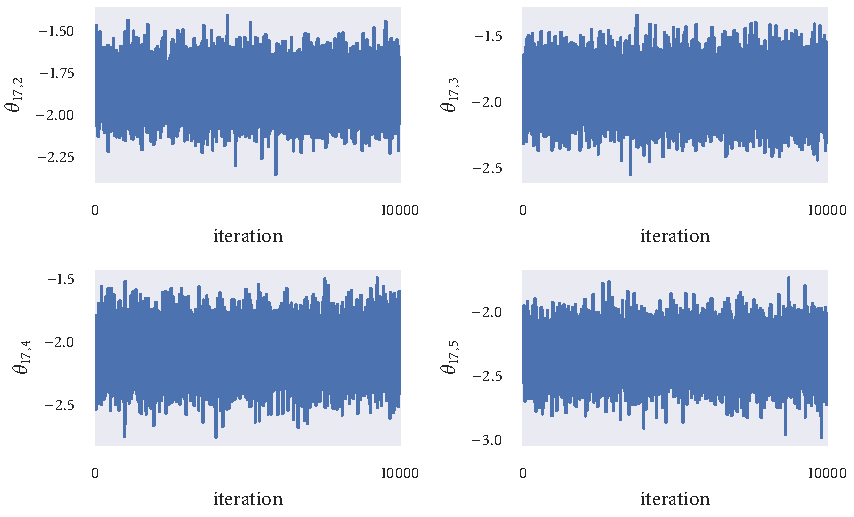
\includegraphics{/data/meetings/2018-05-28/seq05_trace_end_miss_i=17.pdf}
	\caption{Chains over the missing directions of agent $17$, missing from frame $2$ until the end of the sequence.}
	\label{fig:seq05_trace_end_miss_i=17}
\end{figure}
\begin{figure}[tbp]
	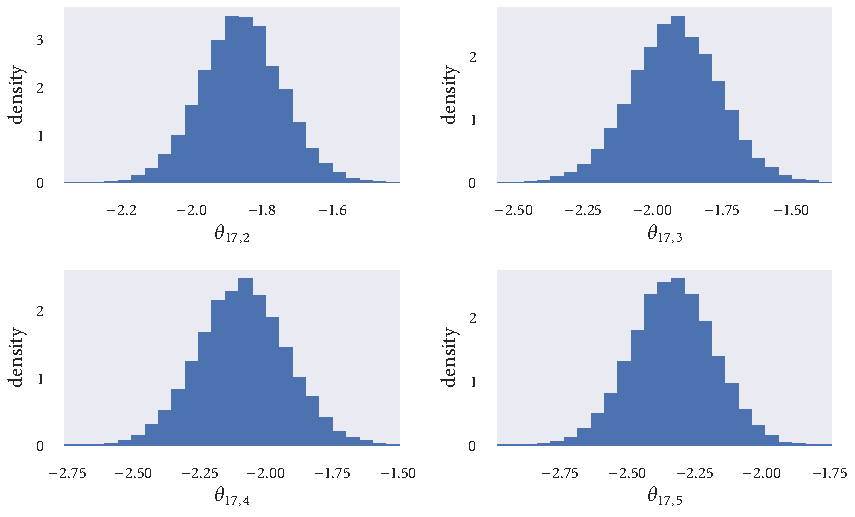
\includegraphics{/data/meetings/2018-05-28/seq05_hist_end_miss_i=17.pdf}
	\caption{Our posterior beliefs about the missing directions of agent $17$, over frames $2$, $3$, $4$ and $5$.}
	\label{fig:seq05_hist_end_miss_i=17}
\end{figure}
\begin{figure}[!tbp]
	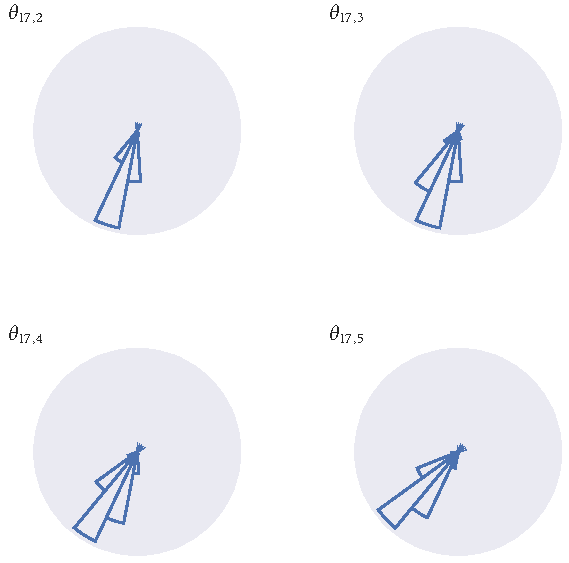
\includegraphics{/data/meetings/2018-05-28/seq05_polar_hist_end_miss_i=17.pdf}
	\caption{Polar histograms showing our posterior beliefs about the missing directions of agent $17$, over frames $2$, $3$, $4$ and $5$.}
	\label{fig:seq05_polar_hist_end_miss_i=17}
\end{figure}
\begin{figure}[!tbp]
	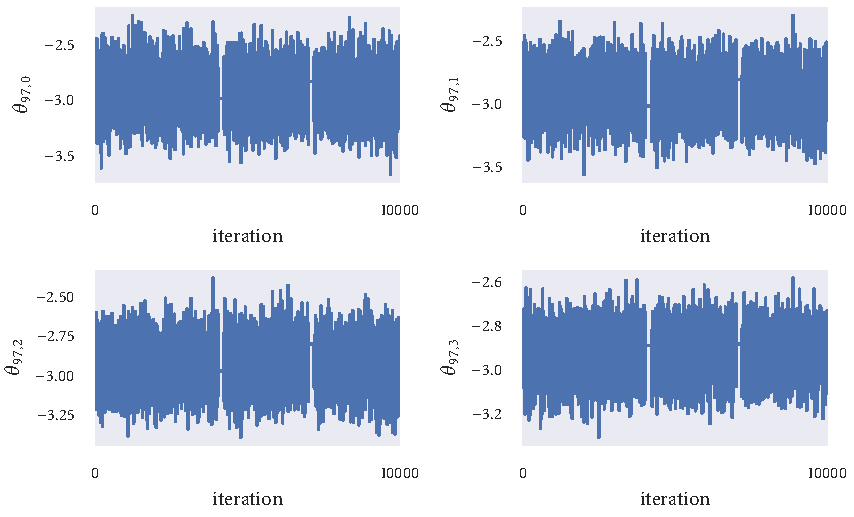
\includegraphics{/data/meetings/2018-05-28/seq05_trace_beg_miss_i=97.pdf}
	\caption{Inferring directions missing at the beginning of a sequence. In particular we show trace plots over agent $97$'s missingness.}
	\label{fig:seq05_trace_beg_miss_i=97}
\end{figure}
\begin{figure}[!tbp]
	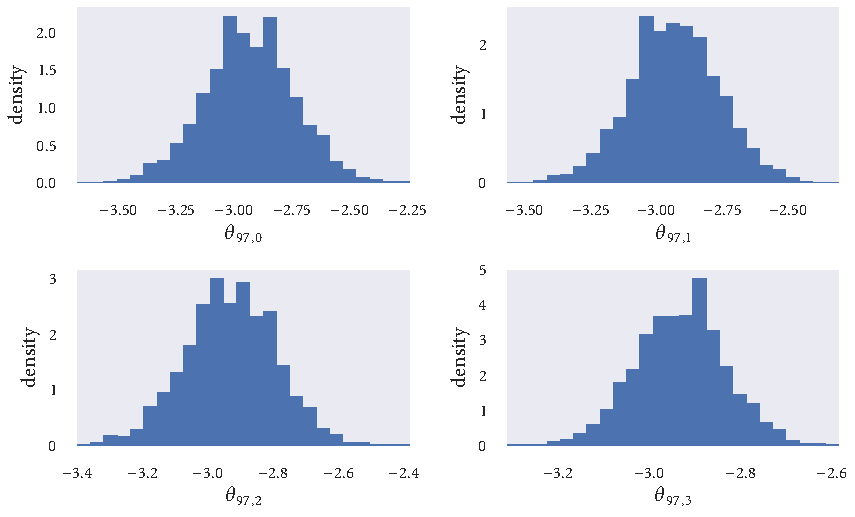
\includegraphics{/data/meetings/2018-05-28/seq05_hist_beg_miss_i=97.pdf}
	\caption{Histogram plots of our posterior beliefs about the missing trajectories of agent $97$.}
	\label{fig:seq05_hist_beg_miss_i=97}
\end{figure}
\begin{figure}[!tbp]
	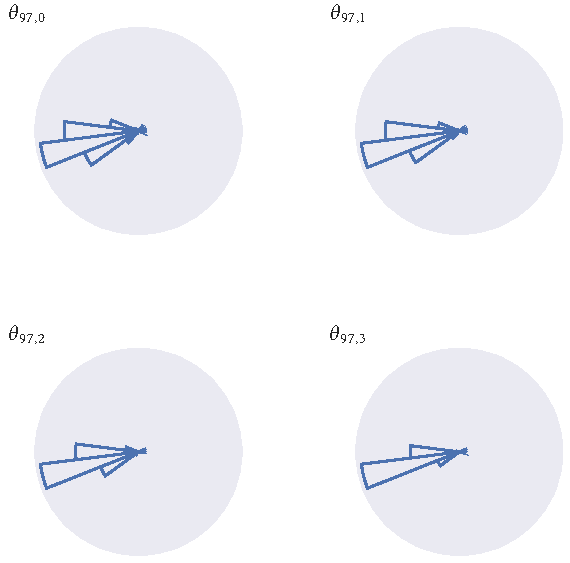
\includegraphics{/data/meetings/2018-05-28/seq05_polar_hist_beg_miss_i=97.pdf}
	\caption{Polar histogram showing our posterior beliefs about the missing directions of agent $97$ at the beginning of the sequence.}
	\label{fig:seq05_polar_hist_beg_miss_i=97}
\end{figure}